\chapter{Chapter 6 --- Phase 3: Diagnosing Learner Behaviour Under
Noise}\label{chapter-6-phase-3-diagnosing-learner-behaviour-under-noise}

Chapter 5 established that label quality matters to an online learner,
and left open which half of the noise is responsible. SZZ makes two
kinds of error --- it invents defects that do not exist, and it misses
defects that do --- and Chapter 4 showed the variants trade one for the
other. Nothing so far indicates which trade is the right one.

This chapter answers \textbf{RQ3}: through what mechanism does label
noise degrade an online learner, and does the learner's
imbalance-handling machinery amplify or absorb each error type?

The chapter uses two complementary designs. A \textbf{dose-response}
experiment injects calibrated noise into clean labels at controlled
doses, giving a clean manipulation on a synthetic gradient. A
\textbf{repair} experiment does the opposite: it takes real B-SZZ labels
and uses the reference to surgically correct one error type at a time,
giving a controlled intervention on real noise. The second is the
stronger design, and it produces the chapter's headline.

\textbf{A result to state at the outset, because it shapes how the
chapter reads.} The hypothesis this project carried into Phase 3 ---
recorded in its own planning documents --- was \emph{false-negative
starvation}: that what hurts an online learner is the true defects a
conservative labeller withholds. \textbf{The controlled experiment
refuted it.} Phase 3 was designed as a genuine test rather than a
confirmation, and it returned the opposite of the expected answer.

\section{6.1 Method}\label{method}

\subsection{6.1.1 The repair experiment}\label{the-repair-experiment}

Take a project's real B-SZZ labels. Using the reference labels,
construct three counterfactual label vectors:

\begin{longtable}[]{@{}
  >{\raggedright\arraybackslash}p{(\linewidth - 2\tabcolsep) * \real{0.5000}}
  >{\raggedright\arraybackslash}p{(\linewidth - 2\tabcolsep) * \real{0.5000}}@{}}
\toprule\noalign{}
\begin{minipage}[b]{\linewidth}\raggedright
Condition
\end{minipage} & \begin{minipage}[b]{\linewidth}\raggedright
Construction
\end{minipage} \\
\midrule\noalign{}
\endhead
\bottomrule\noalign{}
\endlastfoot
\texttt{BSZZ} & The real B-SZZ labels, unmodified \\
\texttt{BSZZ\_fp\_repaired} & B-SZZ with every false positive set to
clean (6,565 labels corrected) \\
\texttt{BSZZ\_fn\_repaired} & B-SZZ with every false negative set to
defective (837 labels corrected) \\
\texttt{oracle} & The reference labels themselves \\
\end{longtable}

Train ORB on each under identical conditions --- same stream, same seed,
same latency model --- and score all four against the reference. The
difference between conditions is attributable to the repair, because
nothing else differs.

\textbf{This is an intervention, not an observation.} Chapter 5's
label-source comparison contrasted whole labelling procedures that
differ in many ways at once. Here a single error type is removed while
everything else is held fixed. That is what licenses a mechanistic
reading.

\textbf{It is also oracle-assisted and therefore not a method.}
Identifying which labels are wrong requires the reference. The repair
experiment measures \emph{what would be recovered if one knew}; Chapter
7 asks whether a learner can approximate it without knowing.

\textbf{Restored false negatives need arrival times.} A commit B-SZZ
labelled clean has no fix linkage, so a restored positive has no natural
delivery date. Arrival times are imputed by sampling the empirical
latency distribution, and \S{}6.2.3 tests whether that imputation drives
the result.

\subsection{6.1.2 The dose-response
experiment}\label{the-dose-response-experiment}

Starting from clean reference labels, inject noise at doses of 5\% to
30\% under four profiles, each calibrated from Chapter 4's measured flip
rates:

\begin{longtable}[]{@{}
  >{\raggedright\arraybackslash}p{(\linewidth - 4\tabcolsep) * \real{0.3333}}
  >{\raggedright\arraybackslash}p{(\linewidth - 4\tabcolsep) * \real{0.3333}}
  >{\raggedright\arraybackslash}p{(\linewidth - 4\tabcolsep) * \real{0.3333}}@{}}
\toprule\noalign{}
\begin{minipage}[b]{\linewidth}\raggedright
Profile
\end{minipage} & \begin{minipage}[b]{\linewidth}\raggedright
Calibration
\end{minipage} & \begin{minipage}[b]{\linewidth}\raggedright
Character
\end{minipage} \\
\midrule\noalign{}
\endhead
\bottomrule\noalign{}
\endlastfoot
\texttt{symmetric} & Equal flip rates both directions & Control --- the
standard assumption \\
\texttt{fp\_heavy} & B-SZZ (\ensuremath{\rho}\ensuremath{_0} 0.263, \ensuremath{\rho}\ensuremath{_1} 0.359) &
False-positive-heavy \\
\texttt{mid} & RA-SZZ (\ensuremath{\rho}\ensuremath{_0} 0.181, \ensuremath{\rho}\ensuremath{_1} 0.562) & Intermediate \\
\texttt{fn\_heavy} & L-SZZ (\ensuremath{\rho}\ensuremath{_0} 0.067, \ensuremath{\rho}\ensuremath{_1} 0.733) &
False-negative-heavy \\
\end{longtable}

\textbf{Dose is defined as the expected fraction of \emph{all} commits
flipped}, with the two class-conditional rates scaled to meet it. \S{}6.2.4
shows that this definition has a consequence severe enough to require
its own analysis.

\subsection{6.1.3 Latency arms}\label{latency-arms}

Each dose-response condition is run under three latency regimes:

\begin{itemize}
\tightlist
\item
  \textbf{\texttt{none}} --- every label delivered immediately after the
  commit is scored. Plain test-then-train, the true no-latency control.
\item
  \textbf{\texttt{uniform}} --- every label delayed by exactly \emph{W}
  = 90 days. A fixed-delay control that removes schedule variation but
  \textbf{not delay}.
\item
  \textbf{\texttt{real}} --- reconstructed arrival times, with late
  defect labels delivered first as wrong clean labels and corrected
  later.
\end{itemize}

The distinction between \texttt{none} and \texttt{uniform} is
load-bearing and was not present in an earlier version of this work.
\S{}6.2.5 records the correction.

\subsection{6.1.4 Instrumentation}\label{instrumentation}

ORB's internals are traced at every learning step: the Poisson rate \ensuremath{\lambda}
applied to the arrival, the boost factor, the running prediction bias,
and the decayed observed class rate. Alongside these, the label
composition of each injected stream is recorded --- how many positives
it carries and how many of them are genuine. This instrumentation is
what turns \S{}6.2.6 from an interpretation into a measurement.

\subsection{6.1.5 Scale and statistics}\label{scale-and-statistics}

21 projects \ensuremath{\times} 10 seeds \ensuremath{\times} 4 profiles \ensuremath{\times} 6 doses \ensuremath{\times} latency arms = 10,080
dose-response records, plus the repair conditions. Tests are paired at
project level (\emph{n} = 21) with Hodges--Lehmann estimates, bootstrap
intervals, matched-pairs rank-biserial and Holm correction, matching
Chapter 5. Both prequential estimators are recorded and
\texttt{mcc\_avg} is primary.

\section{6.2 Results}\label{results}

\subsection{6.2.1 The repair verdict}\label{the-repair-verdict}

\begin{longtable}[]{@{}
  >{\raggedright\arraybackslash}p{(\linewidth - 10\tabcolsep) * \real{0.1667}}
  >{\raggedright\arraybackslash}p{(\linewidth - 10\tabcolsep) * \real{0.1667}}
  >{\raggedright\arraybackslash}p{(\linewidth - 10\tabcolsep) * \real{0.1667}}
  >{\raggedright\arraybackslash}p{(\linewidth - 10\tabcolsep) * \real{0.1667}}
  >{\raggedright\arraybackslash}p{(\linewidth - 10\tabcolsep) * \real{0.1667}}
  >{\raggedright\arraybackslash}p{(\linewidth - 10\tabcolsep) * \real{0.1667}}@{}}
\toprule\noalign{}
\begin{minipage}[b]{\linewidth}\raggedright
Repair
\end{minipage} & \begin{minipage}[b]{\linewidth}\raggedright
HL
\end{minipage} & \begin{minipage}[b]{\linewidth}\raggedright
95\% CI
\end{minipage} & \begin{minipage}[b]{\linewidth}\raggedright
Rank-biserial
\end{minipage} & \begin{minipage}[b]{\linewidth}\raggedright
Projects
\end{minipage} & \begin{minipage}[b]{\linewidth}\raggedright
Holm (global)
\end{minipage} \\
\midrule\noalign{}
\endhead
\bottomrule\noalign{}
\endlastfoot
\textbf{Remove B-SZZ's 6,565 false positives} & \textbf{+0.0402} &
{[}+0.0217, +0.0520{]} & +0.844 & \textbf{17/21} & \textbf{0.0019} \\
Restore B-SZZ's 837 false negatives & \ensuremath{-}0.0012 & {[}\ensuremath{-}0.0089, +0.0080{]} &
\ensuremath{-}0.082 & 8/21 & 1.000 \\
\textbf{The two head to head} & \textbf{+0.0413} & {[}+0.0180,
+0.0575{]} & +0.732 & 17/21 & \textbf{0.0151} \\
\end{longtable}

\textbf{Removing false positives recovers performance. Restoring false
negatives recovers nothing} --- and the interval on that null is tight,
so it is an informative null rather than an underpowered one.

\begin{figure}
\centering
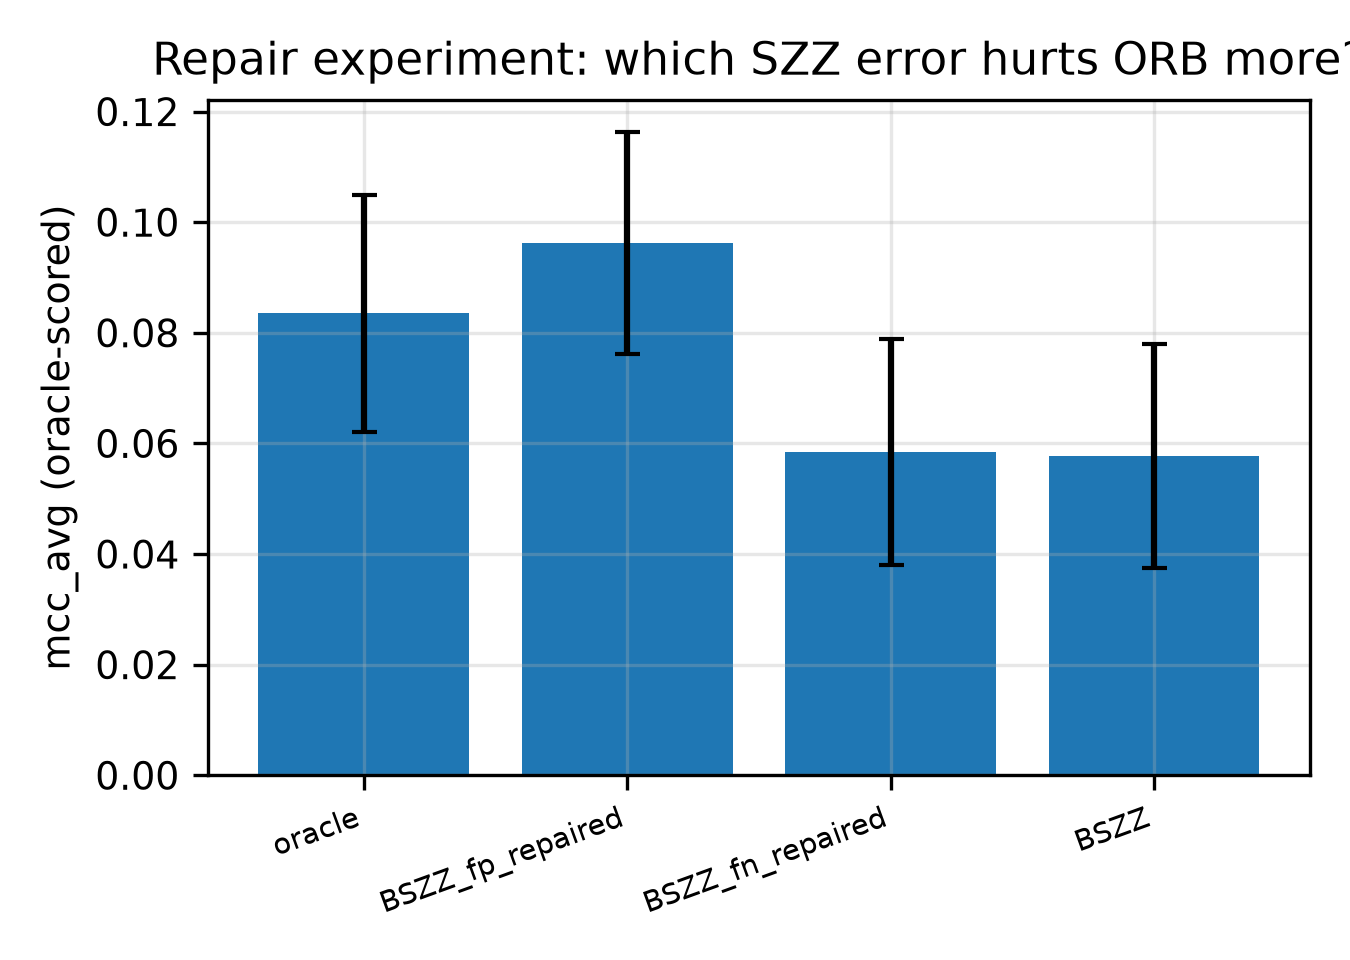
\includegraphics[width=\linewidth,keepaspectratio]{reports/figures/fig_p3_repair_mcc_avg.png}
\label{fig:fig_p3_repair_mcc_avg}
\caption{Repair experiment --- what each surgical correction recovers}
\end{figure}

\textbf{Figure 6.1 --- Reading the figure.} Four bars, left to right:
the reference labels, B-SZZ with its false positives removed, B-SZZ with
its false negatives restored, and unrepaired B-SZZ. Error bars are 95\%
intervals over projects. \textbf{The FP-repaired bar is the tallest ---
above even the reference labels --- while the FN-repaired bar sits level
with unrepaired B-SZZ.} A bar that does not move is the result here, not
a missing one.

A striking detail: FP-repaired B-SZZ reaches a mean of 0.0962 against
the reference labels' own 0.0835. \textbf{A precision-repaired heuristic
outscores the reference itself} (+0.0127, 14/21, \emph{p} = 0.089). For
an online learner under verification latency, label precision is worth
more than label completeness. This is an oracle-assisted upper bound,
not an achievable labeller, and is framed as such.

\subsection{6.2.2 The error-matched control changes what the result
means}\label{the-error-matched-control-changes-what-the-result-means}

B-SZZ carries 6,565 false positives against 837 false negatives --- an
8:1 imbalance. ``Repair all of each'' is therefore not a fair
comparison, and a caveat is not a control. Correcting the \textbf{same
label mass} on both sides:

\begin{longtable}[]{@{}
  >{\raggedright\arraybackslash}p{(\linewidth - 8\tabcolsep) * \real{0.2000}}
  >{\raggedright\arraybackslash}p{(\linewidth - 8\tabcolsep) * \real{0.2000}}
  >{\raggedright\arraybackslash}p{(\linewidth - 8\tabcolsep) * \real{0.2000}}
  >{\raggedright\arraybackslash}p{(\linewidth - 8\tabcolsep) * \real{0.2000}}
  >{\raggedright\arraybackslash}p{(\linewidth - 8\tabcolsep) * \real{0.2000}}@{}}
\toprule\noalign{}
\begin{minipage}[b]{\linewidth}\raggedright
Contrast
\end{minipage} & \begin{minipage}[b]{\linewidth}\raggedright
HL
\end{minipage} & \begin{minipage}[b]{\linewidth}\raggedright
95\% CI
\end{minipage} & \begin{minipage}[b]{\linewidth}\raggedright
Projects
\end{minipage} & \begin{minipage}[b]{\linewidth}\raggedright
Holm
\end{minipage} \\
\midrule\noalign{}
\endhead
\bottomrule\noalign{}
\endlastfoot
FP-repair (matched, \textasciitilde40/project) vs B-SZZ & +0.0024 &
{[}\ensuremath{-}0.0045, +0.0089{]} & 11/21 & 0.864 \\
FP-repair (matched) vs FN-repair (all) & +0.0050 & {[}\ensuremath{-}0.0093,
+0.0176{]} & 14/21 & 0.864 \\
\end{longtable}

\textbf{Removing 837 false positives does nothing. Removing 6,565
recovers +0.040.} At equal corrected mass the two error types are
statistically indistinguishable.

The marginal-value curve reconciles the two results. Repairing false
positives in increments of 25/50/75/100\% gives a roughly linear return
of \textbf{+0.147 MCC per 1,000 labels corrected}, so the
\textasciitilde40 per project that false-negative repair could ever
match predicts +0.006 --- within noise of the +0.002 measured. Nothing
is inconsistent; the effect is simply proportional to volume.

\begin{quote}
\textbf{The claim this supports, stated exactly.} \emph{SZZ's false
positives are what cost the learner, because there are eight times more
of them.} \textbf{Not} \emph{a false positive is individually more
harmful than a false negative.} The second sentence is unsupported by
this experiment and does not appear in this thesis.
\end{quote}

\subsection{6.2.3 The delivery ceiling: content, not
scheduling}\label{the-delivery-ceiling-content-not-scheduling}

A null for false-negative repair admits two readings. The missing labels
may not matter --- or they may be unable to arrive in time to matter,
given that 53\% of defect labels arrive after the decision window.
Restoring them under three delivery regimes, each against its own anchor
so that the contrast isolates restoration from acceleration:

\begin{longtable}[]{@{}
  >{\raggedright\arraybackslash}p{(\linewidth - 6\tabcolsep) * \real{0.2500}}
  >{\raggedright\arraybackslash}p{(\linewidth - 6\tabcolsep) * \real{0.2500}}
  >{\raggedright\arraybackslash}p{(\linewidth - 6\tabcolsep) * \real{0.2500}}
  >{\raggedright\arraybackslash}p{(\linewidth - 6\tabcolsep) * \real{0.2500}}@{}}
\toprule\noalign{}
\begin{minipage}[b]{\linewidth}\raggedright
Delivery regime
\end{minipage} & \begin{minipage}[b]{\linewidth}\raggedright
HL
\end{minipage} & \begin{minipage}[b]{\linewidth}\raggedright
95\% CI
\end{minipage} & \begin{minipage}[b]{\linewidth}\raggedright
Projects
\end{minipage} \\
\midrule\noalign{}
\endhead
\bottomrule\noalign{}
\endlastfoot
Realistic (imputed arrival times) & \ensuremath{-}0.0012 & {[}\ensuremath{-}0.0089, +0.0080{]} &
8/21 \\
Immediate (available at once) & +0.0037 & {[}\ensuremath{-}0.0032, +0.0106{]} &
12/21 \\
At the window boundary (\emph{t} + 90d) & \ensuremath{-}0.0016 & {[}\ensuremath{-}0.0073,
+0.0043{]} & 6/21 \\
\end{longtable}

Three regimes, three nulls. \textbf{Even delivered instantly, the
missing labels recover nothing.} The scheduling explanation is ruled
out; this is a claim about the content of those labels.

\textbf{The null is affirmative, not merely unproven.} A two one-sided
tests (TOST) equivalence procedure --- which asks whether an effect is
small enough to be declared equivalent rather than merely failing to
prove it non-zero --- with a margin declared in advance at \textbf{\ensuremath{\pm}0.02
MCC} (half the measured FP-repair effect) returns \textbf{p = 0.0008}.
False-negative restoration is \emph{equivalent to no repair}.

\subsection{6.2.4 Dose-response, and a parameterisation
trap}\label{dose-response-and-a-parameterisation-trap}

\begin{longtable}[]{@{}llll@{}}
\toprule\noalign{}
Profile & No latency & Fixed 90-day delay & Realistic delay \\
\midrule\noalign{}
\endhead
\bottomrule\noalign{}
\endlastfoot
\texttt{fn\_heavy} & \textbf{\ensuremath{-}0.0553} & \ensuremath{-}0.0370 & \ensuremath{-}0.0363 \\
\texttt{mid} & \ensuremath{-}0.0384 & \ensuremath{-}0.0225 & \ensuremath{-}0.0247 \\
\texttt{fp\_heavy} & \ensuremath{-}0.0313 & \ensuremath{-}0.0196 & \ensuremath{-}0.0205 \\
\texttt{symmetric} & \ensuremath{-}0.0286 & \ensuremath{-}0.0177 & \ensuremath{-}0.0222 \\
\end{longtable}

\emph{(MCC lost per 10\% of labels flipped, fitted on non-degenerate
cells only.)}

At matched dose, false-negative-heavy noise degrades the learner fastest
--- which appears to contradict \S{}6.2.1 and does not.

\begin{figure}
\centering
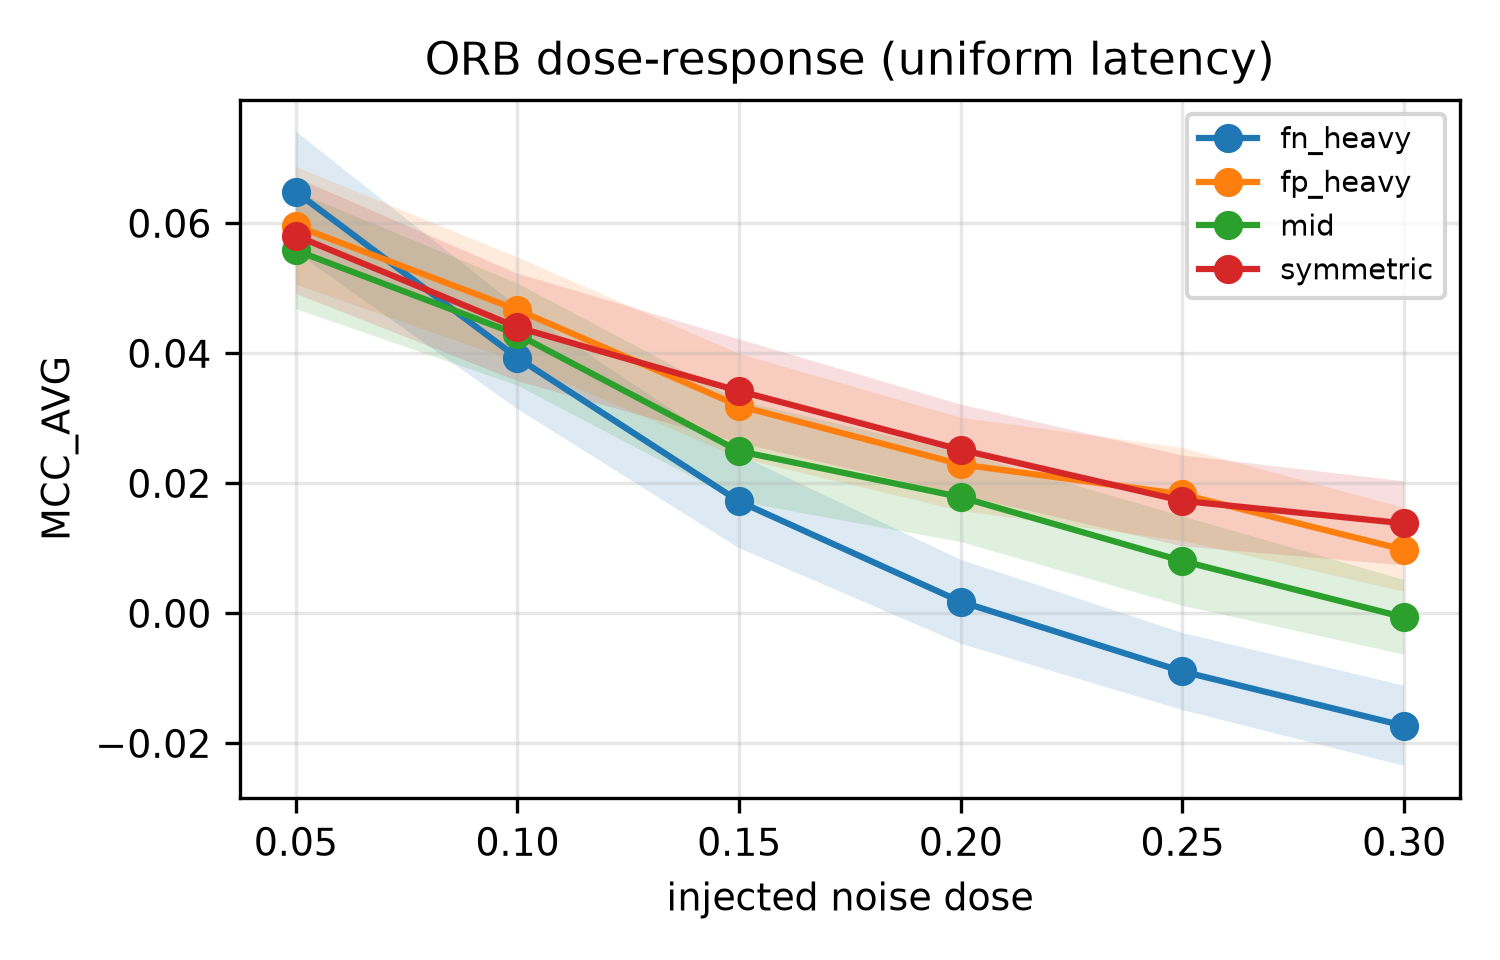
\includegraphics[width=\linewidth,keepaspectratio]{reports/figures/fig_p3_dose_mcc_avg_uniform.png}
\label{fig:fig_p3_dose_mcc_avg_uniform}
\caption{ORB dose-response by noise profile}
\end{figure}

\textbf{Figure 6.2 --- Reading the figure.} Each line is one noise
profile as the injected dose rises; shaded bands are 95\% intervals. The
FN-heavy line (blue) falls fastest and crosses zero --- but see the
caution below, which is the reason its steepness cannot be read as
severity.

\textbf{Dose is a fraction of all commits.} At equal dose the FN-heavy
profile strips far more of the 8.5\% minority class. Measured retention
of genuine defect labels:

\begin{longtable}[]{@{}lllllll@{}}
\toprule\noalign{}
Profile & 0.05 & 0.10 & 0.15 & 0.20 & 0.25 & 0.30 \\
\midrule\noalign{}
\endhead
\bottomrule\noalign{}
\endlastfoot
\texttt{fn\_heavy} & 0.720 & 0.440 & 0.183 & 0.056 & 0.010 &
\textbf{0.000} \\
\texttt{fp\_heavy} & 0.938 & 0.868 & 0.804 & 0.739 & 0.669 & 0.601 \\
\end{longtable}

\begin{quote}
\textbf{At the highest dose the FN-heavy stream is not empty --- it is
poisoned.} It still carries roughly 204 positive labels, \emph{every one
of them false}, because the L-SZZ profile also flips clean commits
upward and the majority class is large enough to supply plenty. Fitting
a straight line through that region understates the slope and invites a
comparison the design cannot support, so slopes are fitted only on cells
retaining genuine defect labels, with the survival table published
alongside.
\end{quote}

\textbf{The two findings are reconciled by the denominator, and the
reconciliation is the substantive point of this chapter.} Per
\emph{label flipped}, false-negative noise is more damaging, because
defect labels are scarce. Per \emph{error actually present in real SZZ
output}, false-positive noise dominates, because B-SZZ produces eight
times more of them.

\subsection{6.2.5 Latency masks label quality --- a
correction}\label{latency-masks-label-quality-a-correction}

An earlier version of this work concluded that latency does \textbf{not}
compress sensitivity to label quality. \textbf{That conclusion was
wrong, and the error was in the design rather than the arithmetic.} The
comparison ran between the \texttt{uniform} and \texttt{real} arms ---
\emph{both heavily delayed}, differing only in arrival schedule. It
tested schedule sensitivity and could not test masking at all.

Against a true no-latency control the picture reverses. Slopes are
approximately \textbf{50\% steeper} without latency, and the separation
between the FN-heavy and FP-heavy profiles widens from \ensuremath{-}0.0158 (real)
and \ensuremath{-}0.0174 (uniform) to \textbf{\ensuremath{-}0.0240} (none) --- roughly 40\% better
separated. Mean MCC at the lowest dose is 0.0995 without latency against
0.0525 with it.

\begin{figure}
\centering
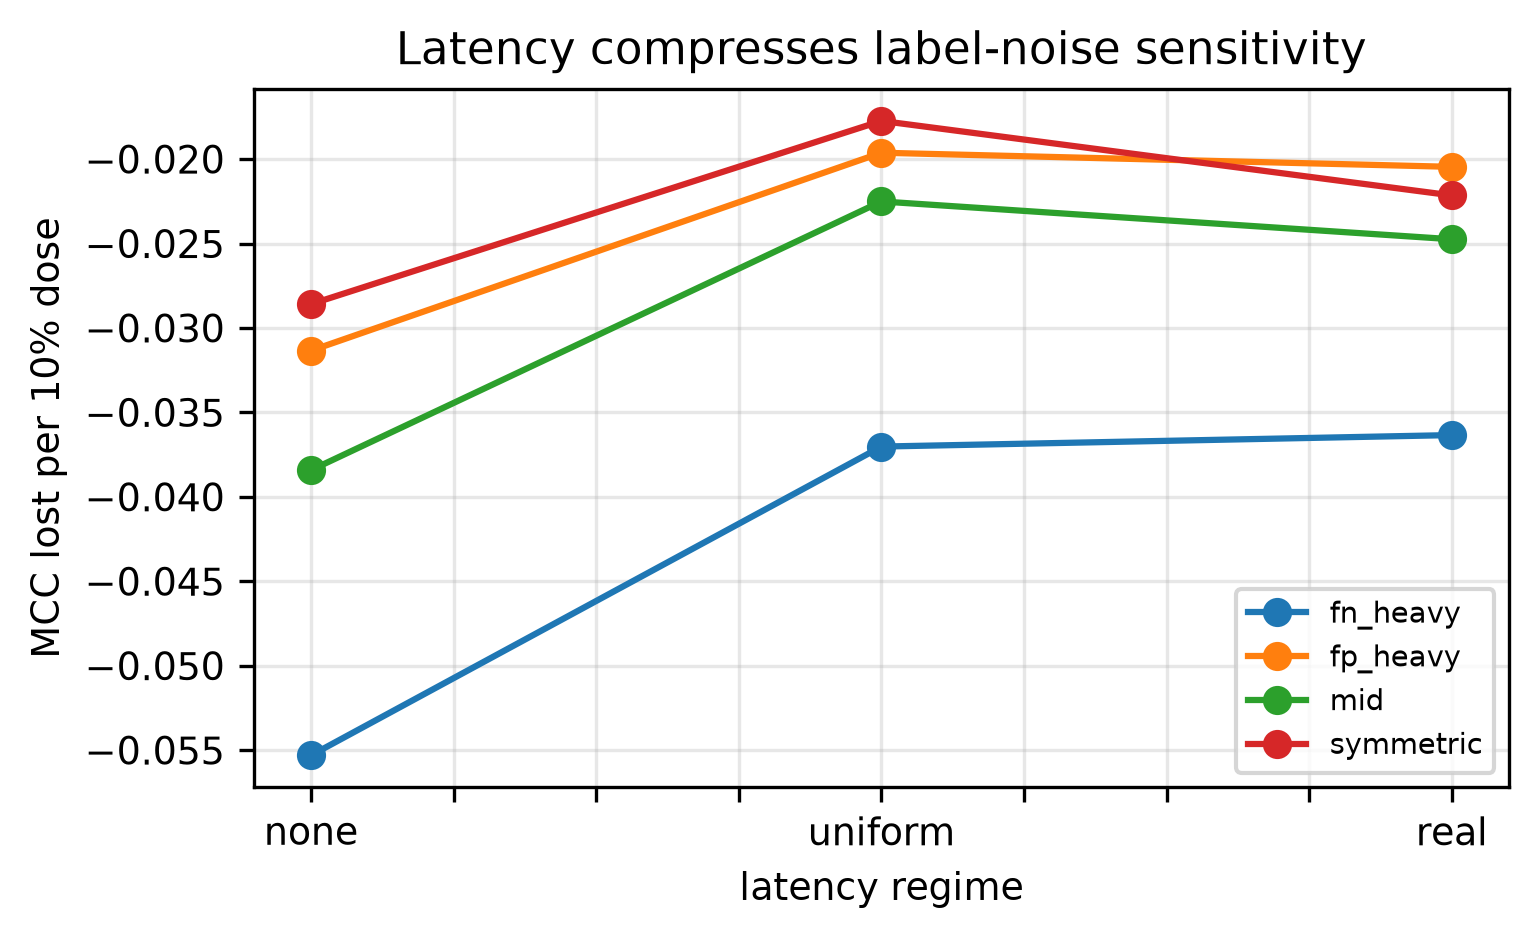
\includegraphics[width=\linewidth,keepaspectratio]{reports/figures/fig_p3_latency_arms.png}
\label{fig:fig_p3_latency_arms}
\caption{Dose slopes under three latency regimes}
\end{figure}

\textbf{Figure 6.3 --- Reading the figure.} Each line is a noise
profile; the x-axis moves from no latency, through a fixed 90-day delay,
to realistic delay. The lines both flatten and converge as latency
increases --- flattening is the compression, converging is the loss of
discrimination between label sources.

\textbf{Verification latency both lowers the ceiling and flattens the
response to label quality.} Under deployment conditions, better labels
buy less than they would in a batch setting --- which is an independent
reason to expect batch-measured noise studies to overstate what label
cleaning can deliver.

\subsection{6.2.6 The mechanism: the boost compensates for scarcity, not
for
correctness}\label{the-mechanism-the-boost-compensates-for-scarcity-not-for-correctness}

ORB handles class imbalance by oversampling: each arriving example is
presented to each ensemble member \emph{k} \textasciitilde{} Poisson(\ensuremath{\lambda})
times, with \ensuremath{\lambda} for the minority class set from the running observed class
rate as \ensuremath{\lambda}\ensuremath{_1} = (1 \ensuremath{-} r\ensuremath{_1})/r\ensuremath{_1}, and further amplified when the model's recent
predictions are biased against the minority class.

The instrumentation makes the consequence measurable.

\begin{figure}
\centering
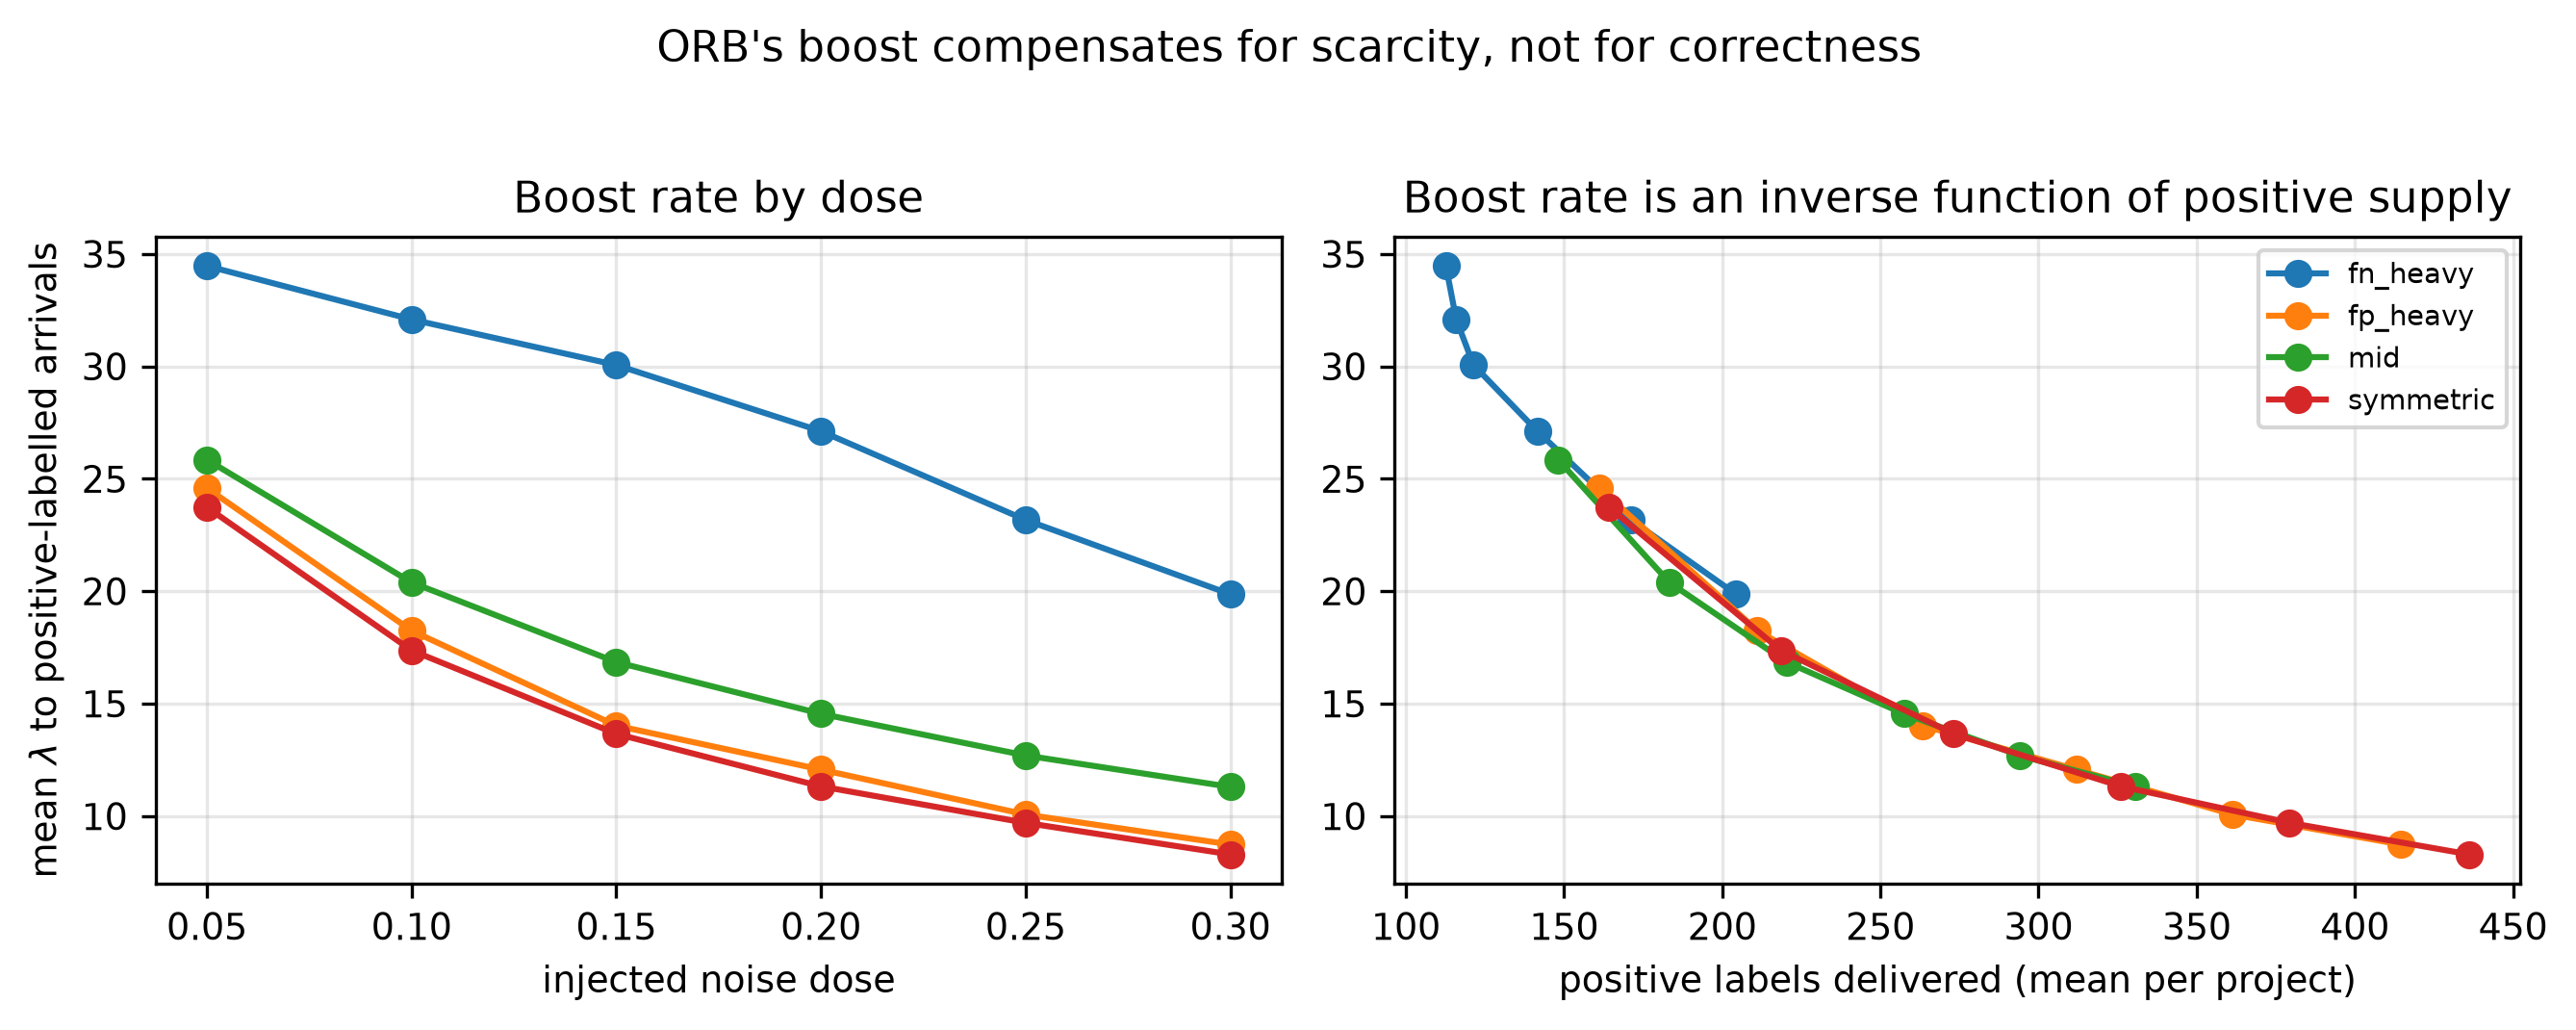
\includegraphics[width=\linewidth,keepaspectratio]{reports/figures/fig_p3_lambda_compensation.png}
\label{fig:fig_p3_lambda_compensation}
\caption{Boost rate against delivered defect-label supply}
\end{figure}

\textbf{Figure 6.4 --- Reading the figure.} \emph{Left:} the learner's
oversampling rate against injected noise dose, one line per profile ---
the profiles separate, so \ensuremath{\lambda} is not a function of dose alone.
\emph{Right:} the same rate against how many defect labels the stream
actually delivers. \textbf{The right panel collapses onto a single
curve}, which is the finding: \ensuremath{\lambda} is a function of label supply and of
nothing else. The mean \ensuremath{\lambda} applied to defect-labelled arrivals is an
almost perfect inverse function of how many such labels the stream
delivers:

\begin{itemize}
\tightlist
\item
  \textbf{Spearman \ensuremath{\rho} = \ensuremath{-}1.000} across profiles at matched dose
\item
  \ensuremath{\rho} = \ensuremath{-}0.70 to \ensuremath{-}0.87 within each profile
\end{itemize}

\begin{longtable}[]{@{}lll@{}}
\toprule\noalign{}
Profile & Defect labels delivered (mean/project) & Mean \ensuremath{\lambda} \\
\midrule\noalign{}
\endhead
\bottomrule\noalign{}
\endlastfoot
\texttt{fn\_heavy} @ dose 0.05 & 113 & \textbf{34.5} \\
\texttt{symmetric} @ dose 0.05 & 164 & 23.7 \\
\texttt{fn\_heavy} @ dose 0.30 & 204 \emph{(all false)} & 19.9 \\
\texttt{symmetric} @ dose 0.30 & 436 & 8.3 \\
\end{longtable}

\begin{quote}
\textbf{ORB's boost compensates for defect-label \emph{scarcity}, not
for false negatives --- it cannot tell the difference.} It amplifies
whatever positive labels arrive, and amplifies them hardest exactly when
they are rarest.
\end{quote}

This is the mechanism the chapter was looking for, and it explains both
halves of the result:

\textbf{Why restoring false negatives recovers nothing.} The learner has
already compensated for their absence. Removing defect labels raises \ensuremath{\lambda}
on those that remain, which partially replaces the lost gradient mass.
Adding the missing labels back supplies something the mechanism had
already approximated.

\textbf{Why removing false positives recovers a great deal.} A false
positive receives the same amplification as a true one --- the boost has
no facility for discounting a label it does not trust. \textbf{The
machinery that corrects class imbalance is the machinery that magnifies
wrong labels}, and it magnifies them hardest precisely when defect
labels are scarcest, which under verification latency is always.

\section{6.3 Discussion --- answering
RQ3}\label{discussion-answering-rq3}

\textbf{Through what mechanism does label noise degrade an online
learner?} Through amplification, not through starvation. ORB's
oversampling rate is set by the observed rate of defect labels, so it
responds to the \emph{quantity} of positive labels and is blind to their
\emph{quality}. False positives are therefore not merely learned ---
they are learned harder than a balanced learner would learn them, and
hardest under exactly the conditions that make deployment realistic.

\textbf{Does the learner amplify or absorb each error type?} It absorbs
false negatives, by construction: their absence raises \ensuremath{\lambda}, which
partially compensates. It amplifies false positives, also by
construction, and has no mechanism to do otherwise.

\textbf{Which error dominates in practice?} False positives ---
\textbf{because of their volume, not their unit severity.} This is the
distinction the error-matched control enforces, and it is the difference
between a claim this thesis can defend and one it cannot.

\subsection{6.3.1 Design requirements extracted for Phase
4}\label{design-requirements-extracted-for-phase-4}

\begin{enumerate}
\def\labelenumi{\arabic{enumi}.}
\tightlist
\item
  \textbf{Target false positives, not false negatives.} Restoring
  missing defect labels is equivalent to no repair. This retires the
  rescue mechanism Phase 4 was originally designed around.
\item
  \textbf{Operate at volume.} The benefit is roughly linear at +0.147
  MCC per 1,000 corrected labels, so an intervention touching a few
  dozen labels per project will do nothing detectable.
\item
  \textbf{Expect the benefit to track each label source's false-positive
  count.} This is a falsifiable ordering prediction across six variants
  whose counts are known in advance, and it becomes Phase 4's sharpest
  test.
\item
  \textbf{Anticipate interference with the boost.} Because \ensuremath{\lambda} is an
  inverse function of delivered defect-label supply, any filter that
  suppresses positives raises \ensuremath{\lambda} for the survivors. Whether that helps or
  hurts is not obvious and must be registered as a risk rather than
  assumed.
\item
  \textbf{Guard the clean-label case.} Nothing here shows a filter can
  tell a false positive from a correct label the model has not yet
  learned. Non-degradation on clean labels is the acceptance bar, not a
  secondary check.
\end{enumerate}

\subsection{6.3.2 What this chapter licenses, and what it does
not}\label{what-this-chapter-licenses-and-what-it-does-not}

\textbf{Licensed.} That the volume of SZZ's false positives is what
costs an online learner performance on this corpus; that restoring its
false negatives is equivalent to no repair under every delivery regime
tested; that verification latency compresses sensitivity to label
quality; that ORB's oversampling responds to label quantity and is blind
to label quality.

\textbf{Not licensed.} That a false positive is individually more
harmful than a false negative --- the error-matched control rules this
out. That these conclusions transfer to learners without an
imbalance-driven oversampling mechanism; the mechanism identified is
specific to that architecture. That a deployable method can capture the
measured +0.040, since every repair here is oracle-assisted.

The last of these is Chapter 7's question, and its answer is not the one
the design requirements above would predict.
